\pagenumbering{arabic}
\section{绪论}

\subsection{研究背景及意义}
\subsubsection{研究背景}

医学图像是指利用医学成像技术生成的视觉图像,涵盖计算机断层扫描(CT)、磁共振成像(MRI)、超声成像(US)等多种成像模态,通过分析其提供的组织结构、解剖细节及病理信息,放射科医师和内科医师可以快速准确地进行诊断。对医学图像进行图像分割是分析的关键步骤之一,它涉及将图像划分为解剖结构或病灶区域(如器官、组织或病变)相对应的不同区域,这种支持肿瘤定位、器官边界划定的分割可以精确解释医学图像,为临床应用中的准确诊断、术前规划和定量分析奠定了基础\cite{panayides2020}。鉴于其重要性和对临床结果的直接影响,医学图像分割的准确性成为现代医疗健康系统工作中不可或缺的要求。然而,当前临床实践中大量依赖放射科医生手动标注分割图像,不仅耗时费力,还存在一定的主观性和一致性问题。尤其在高分辨率三维图像中,手动标注的工作量极大,容易引发标注者疲劳、遗漏或偏差,进而影响诊断质量。因此,伴随着医学图像数量的激增,研究高效、自动化且高精度的医学图像分割方法,不仅能偶减轻医生负担、提升标注一致性,更在促进智能辅助诊疗系统落地中扮演着不可替代的角色。

\begin{figure}[h]
    \centering
    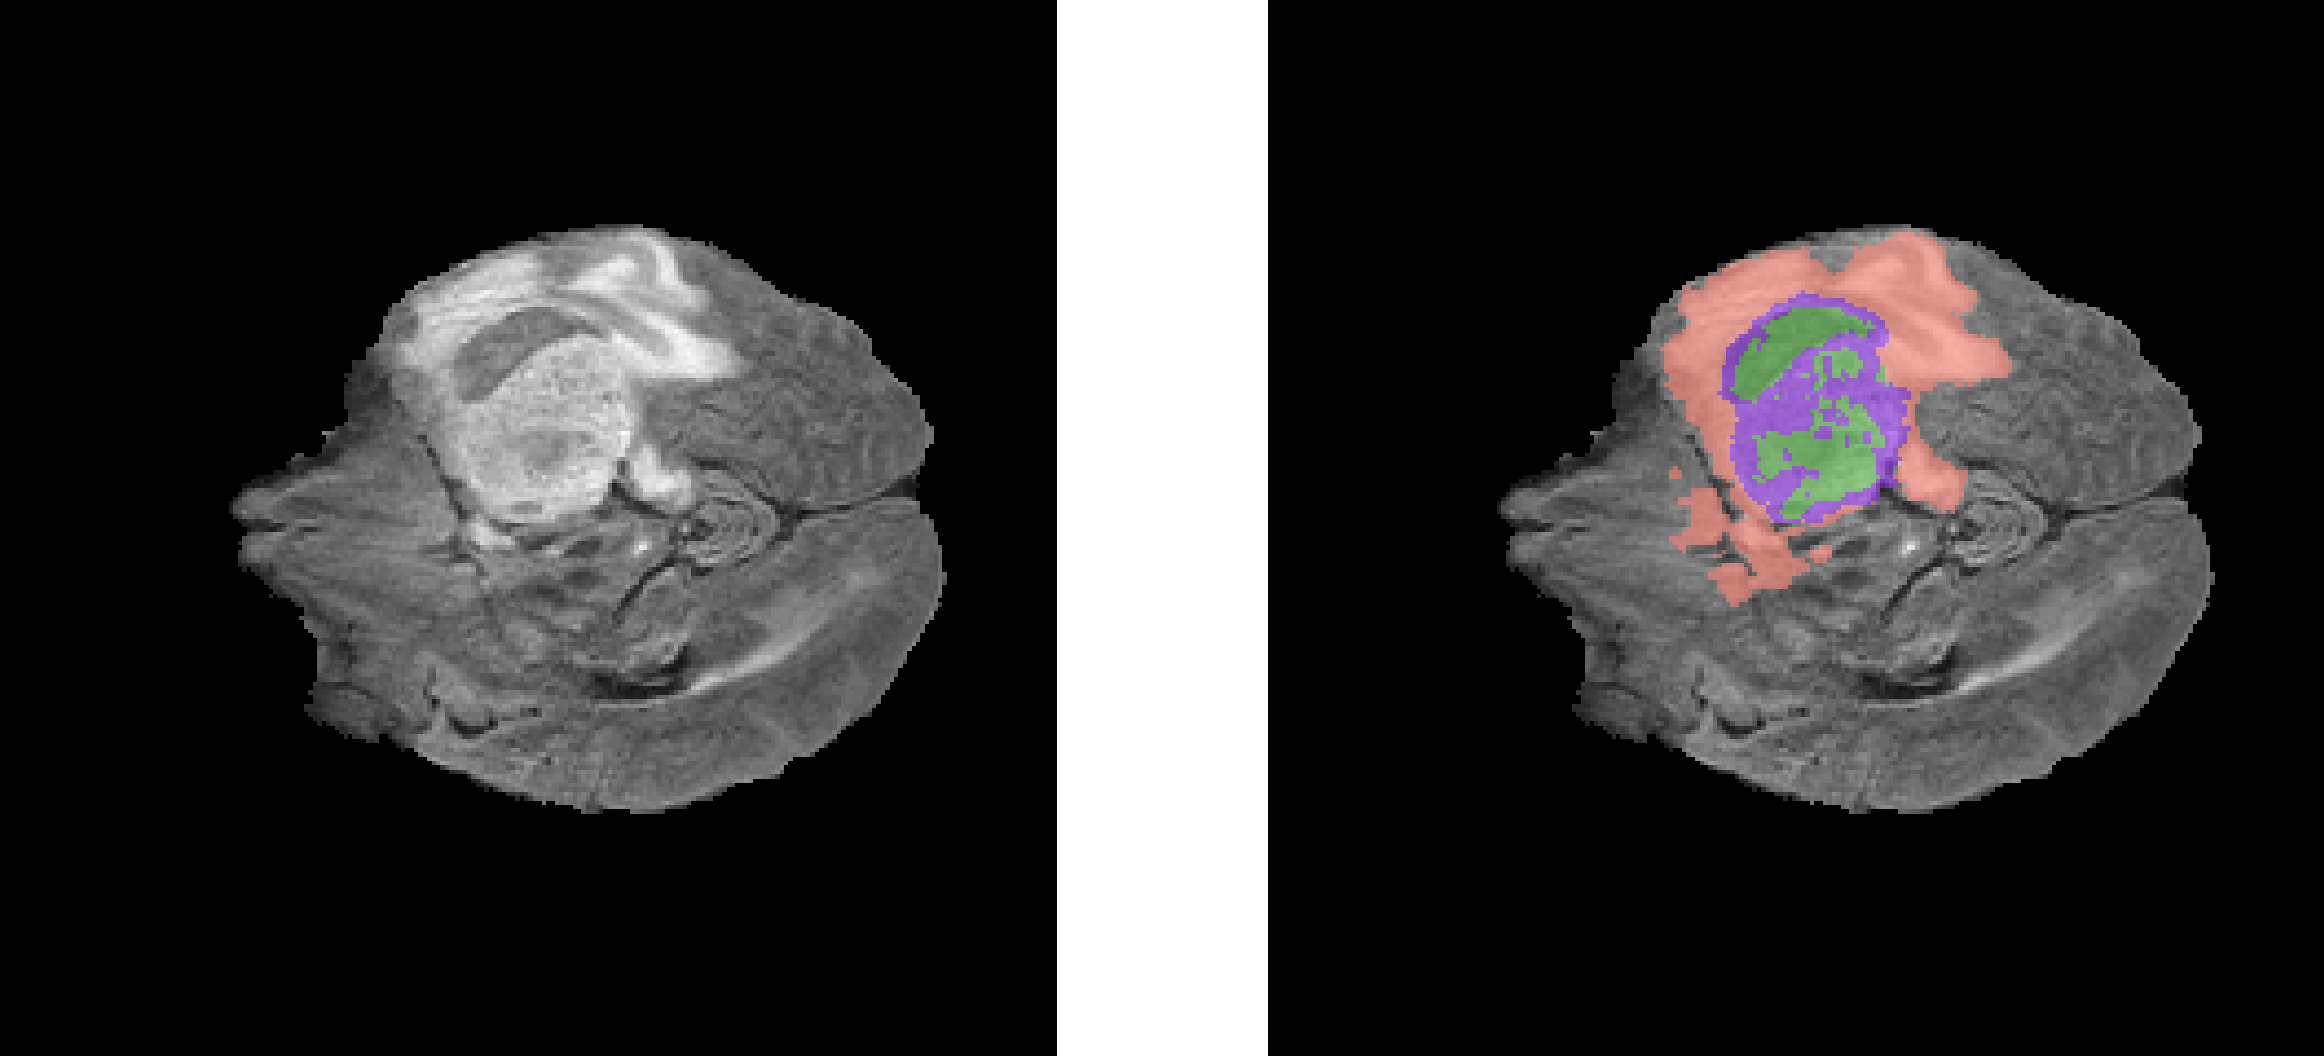
\includegraphics[width=0.77\textwidth]{fig/flair_and_mask.png}
    \caption{脑部MRI图像(左)及对应肿瘤手工标注结果(右)}
    \label{brian_tumor}
\end{figure}

在医学图像分割发展的早期阶段,主要借助阈值分割、区域生长、边缘检测、聚类分割等传统算法来开展组织、器官以及病灶区域的识别与提取工作,这些方法大多依靠人工设计特征或者强先验假设,依据像素灰度、边缘梯度、区域一致性等低层视觉信息构建规则,有较高的可解释性以及计算效率。然而医学图像 成像过程中引入的噪声干扰、患者间器官形态的个体差异与非线性形变、边界信息的模糊,以及多模态成像之间强度分布的较大差异等特点\cite{mohdsagheer2020},致使依赖简单灰度或梯度判断的传统方法难以精确分割目标区域。同时,传统分割算法大多时候需要依赖专业人员进行参数调整、种子点选择或者后处理操作,操作流程繁杂、效率不高,严重制约了其在大规模医学影像分析系统中的推广与部署。基于上述原因,尽管传统图像分割方法在特定条件下仍然有参考价值,但其在面对复杂医学图像时的表达能力与适应性明显不足,急需更具自动学习能力和结构建模能力的先进方法来突破其局限。

随着神经网络以及深度学习快速发展并得到应用,以卷积神经网络作为典型代表的深度学习方法,于图像分类、检测与分割等计算机视觉任务里收获了突破性成果,其有的端到端特征提取能力以及强大的表征学习能力,促使图像分割任务从传统手工设计特征的模式,朝着自动特征学习与高维特征建模的方向转变。最早把深度学习运用到图像分割的代表性模型有全卷积神经网络和SegNet等\cite{shelhamer2016,badrinarayanan2016},全卷积神经网络凭借去掉全连接层,把图像转化成像素级别的类别预测图,是端到端分割网络的起始,SegNet在此基础上引入池化索引来进行上采样,提高了细节还原能力。借助卷积神经网络等技术,深度学习方法依靠其出色的图像分割性能和适应性,在医学图像分割领域渐渐替代了传统算法的位置。不过这些早期模型在医学图像场景中依旧面临一些局限:对弱边界区域识别不够敏感,对结构复杂或者形变剧烈的解剖区域分割精度存在限制,并且对小样本训练数据依赖程度较高,泛化能力不足等。

面对医学图像存在小样本、边界模糊等难题,Ronneberger等人\cite{ronneberger2015}在2015年提出了经典的U-Net模型。U-Net采用编码器和解码器结构,前半部分借助卷积和池化来提取高层语义特征,后半部分凭借反卷积逐步恢复空间分辨率。并且网络利用跳跃连接把编码器里浅层的高分辨率特征与解码器中对应层的特征图拼接融合,有效弥补了深层语义特征里局部细节的缺失。在ISBI细胞分割挑战赛中,U-Net因其出色的结构设计,以较大优势获得冠军。U-Net的提出标志着深度学习在医学图像分割领域广泛应用的开端,还为融合传统知识与深度模型提供了范式基础,奠定了现代医学图像分割算法的主流框架。

\begin{figure}[h]
    \centering
    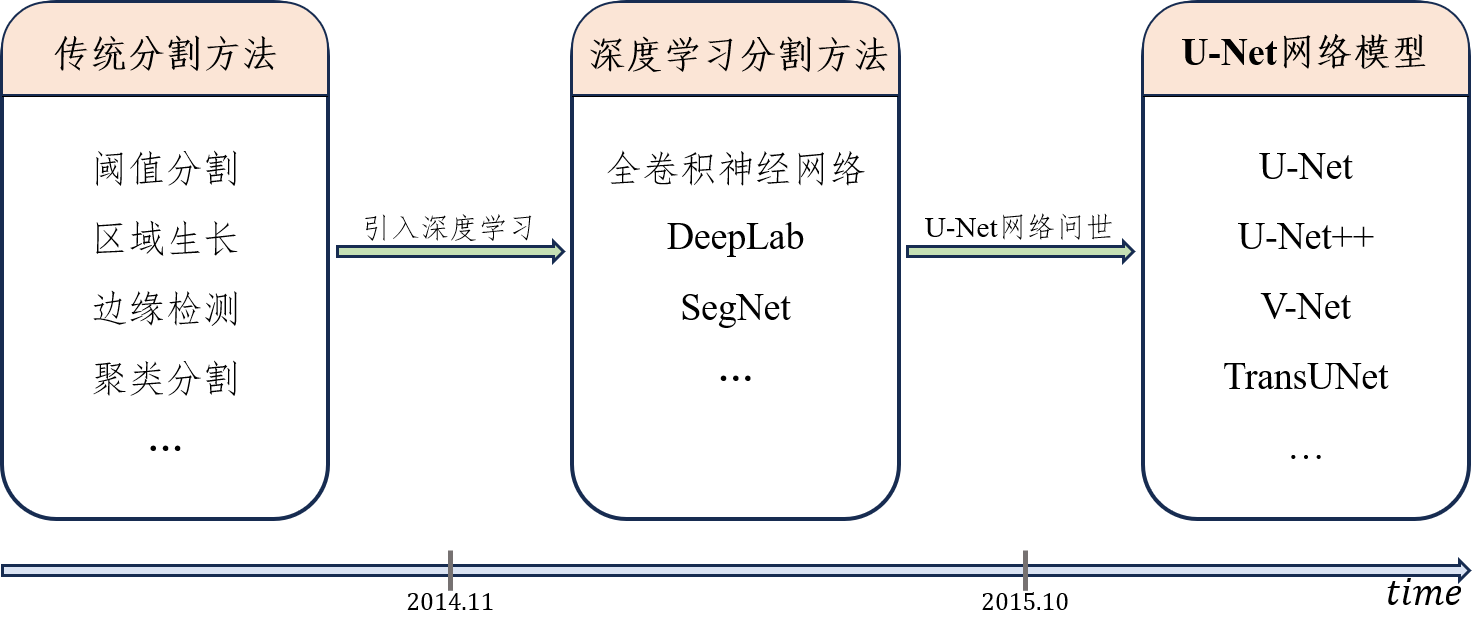
\includegraphics[width=\textwidth]{fig/develepment_of_seg.png}
    \caption{医学图像分割方法发展脉络}
    \label{develop_seg}
\end{figure}

虽然U-Net在医学图像分割方面收获了极大成功,然而随着临床场景变得变得日益复杂以及精度要求不断提升,原始U-Net在诸多实际应用里还是存在着十分突出的局限性:当面对多个病灶区域彼此靠近或者重叠的情况,模型很难有效地分辨各个目标,容易出现融合或者漏检的现象,对于尺寸比较小的病灶,由于其在特征图里容易被下采样过程压缩甚至丢失,致使分割结果里频繁出现漏检,另外,U-Net对输入图像的质量也比较敏感,在存在伪影、噪声或者成像伪差等干扰的时候,模型的鲁棒性很难得到保证\cite{azad2024}。

针对上诉U-Net模型在分割精度和模型鲁棒性等方向存在的局限性,现有研究已经在多个方向上取得了不错的进展\cite{krithikaaliasanbudevi2022},例如Oktay等人\cite{oktay2018}在他们提出的Attention U-Net模型中,在跳跃连接中引入注意力机制来增强模型对分割目标区域的响应,同时抑制无关背景噪声的干扰。这些研究进展及其改进方向将在1.2节中展开叙述。本研究在现有研究的基础上,整合了多个有效的改进方案,旨在构建一个分割性能更高,泛化能力更强的改进模型。

\subsubsection{研究意义}

本研究的学术意义主要体现在以下几个方面:

就理论价值角度而言,对U-Net模型展开系统性改进,以此提升其针对复杂结构、细粒目标以及低对比度区域的建模能力,这可解决医学图像分割里的多个核心难题,还可以为设计有更强表达能力与泛化能力的深度模型开拓新的思路,改进后的模型架构以及训练策略在结构设计、信息流建模以及优化方法等方面都有一定创新性,对医学图像语义分割任务的理论体系起到补充作用,也为应对小样本条件下的训练、提升模型鲁棒性及解释性等问题提供了有借鉴价值的解决办法。

从应用价值角度来看,在实际临床中,医学图像分割是众多关键诊疗环节的基础,在肿瘤检测、器官分割、病灶定量评估等任务中占据核心地位,提高分割模型的精度与效率,可有效辅助医生快速且准确地定位病灶区域,像脑肿瘤、乳腺结节、血管斑块等,减少漏诊误判情况,提升诊断一致性,减轻医生的工作负担。在多目标重叠、边界模糊等复杂场景中,基于改进U-Net的高性能模型可为医生提供更清晰、准确的辅助分割结果,提升临床诊疗的整体质量,高质量的自动分割模型可广泛应用于放射治疗中的靶区勾画、术前路径规划、术中导航与术后评估中,减少对经验丰富医生的高度依赖,降低因人工勾画不一致带来的手术误差与放疗剂量偏差,为治疗过程的标准化与精细化提供技术保障。另外结合患者的个体影像特征与多模态医疗数据,本研究成果也会为实现个性化医疗提供支持,比如用于移植器官体积与形状评估、疗效追踪、慢病进展预测等,可推动以患者为中心的精准医疗落地。

从社会价值角度出发,依据WHO《世界健康统计2025》报告\cite{who2021stats},2023年全球医疗人员缺口高达1470万人,预计2030年仍会维持在1110万人以上,在非洲与东地中海占据近七成。这一结构性短缺为医学图像自动化分割等智能化辅助技术在全球范围内的应用提供了迫切现实背景,面向基层医疗或资源匮乏地区,轻量化、高精度、可部署性的医学图像分割模型可构建低成本的智能辅助诊断系统,缓解医资不均、专家短缺等公共卫生难题,推动普惠医疗的发展,本研究拥有一定的学术理论价值,也有广泛且深远的临床实践与社会应用前景。

\subsection{国内外研究现状}

自2015年Ronneberger等人提出U-Net以来,被引用超过73600次,其凭借高效的特征提取与恢复能力,在医学影像的任务中取得了广泛的应用,成为了医学图像分割领域最广泛使用的架构之一。然而,传统U-Net仍然存在显著的局限性:在全局信息建模和边界细化方面不足;感受野有限,难以捕捉全局上下文,对结构复杂或背景噪声大的区域理解不足;模型冗余大,计算成本高等。因此,近年来国内外学者针对这些问题以及不同的应用场景,在原始U-Net网络的基础上,通过优化结构、引入注意力机制、融合多尺度特征等方法,提出了多种改进模型。这些改进已在多篇相关综述类文章中被系统总结\cite{azad2024,krithikaaliasanbudevi2022,wang2023},下文中将根据Azad等人提出的U-Net变体分类法\cite{azad2024},对国内外学者的研究现状进行概述。

\subsubsection{国外研究现状}

当前国际学术界在医学图像分割领域主要围绕U-Net架构的改进与创新展开研究,重点研究方向包括:多尺度特征融合优化、混合架构创新和多模态处理突破。

多尺度特征融合策略可以通过组合来自不同空间分辨率或感受野范围的特征,增强网络对不同大小、模糊边界目标的识别能力。因此,许多改进模型通过改进U-Net网络的跳跃连接以增强U-Net网络的多尺度特征融合,以提高其上下文建模能力。Zhou等人\cite{zhou2018}提出了Unet++模型,通过密集跳跃连接优化特征重用,相较于U-Net网络只融合同层级的编码器和解码器特征图,UNet++实现了更精细的多尺度特征融合,改善了小目标与弱边界的分割性能。OKtay等人\cite{oktay2018}最早将注意力机制引入U-Net,通过在跳跃连接中引入注意力门(Attention Gates, AGs),他们提出了attention U-Net模型。attention U-Net可以根据高层语义信息和浅层特征图联合计算注意力权重,增强对目标区域的响应抑制无关区域的响应,同时避免冗余的模型结构。通过在跳跃连接中引入双向卷积LSTM(long-term-short-term-memory)模块,Azad等人\cite{azad2019}提出了BCDU-Net模型,将来自编码器和解码器的特征图在双向卷积LSTM中进行组合,提供了丰富的同时包含语义和局部信息的特征图。

在对称的编码-解码器结构中,通过编码器提取多层次语义特征并压缩空间信息,解码器逐步恢复分辨率并融合浅层细节,可以实现对目标区域的精准分割。相较于U-Net采用卷积神经网络作为编码-解码结构层,许多研究者通过采用或结合不同的网络层来构建U-Net,以提高网络的语义分割能力。受残差网络的启发,Drozdzal等人\cite{drozdzal2016}提出了residual U-Net网络,包含编码-解码层的长跳跃连接和卷积网络层之间跨层的短跳跃连接,实现了相较于原始U-Net网络更快的训练收敛。同样地,Milletari等人\cite{milletari2016}所提出的V-Net模型,是以3D残差块作为网络的主体部分,该模型可达成对3D图像更为快速且精准的分割效果,Ibtehaz等人\cite{ibtehaz2020}提出的MultiResUnet基于Inception块构建,它借助并行堆叠3×3、5×5以及7×7卷积核来捕获多尺度特征,在维持参数效率的状况下,有效提升了模型对于多尺寸目标的适应能力。Karaali等人\cite{karaali2022}利用密集残差块提出了Residual Dense-Net,使得特征在局部密集连接中得以传播的同时还拥有跨单元的残差路径,提升了模型的表达能力以及训练稳定性。
% 补充例子

位于编码器和解码器中间最底层的瓶颈区域(Bottleneck),代表着输入数据最深层次的语义,其分辨率最低,通道数却是最多的,对整体性能有着极大的影响。许多研究凭借改进瓶颈区域来提升模型对复杂结构的建模能力,以此弥补压缩所造成的信息损失,其中不少研究者选择引入注意力机制,比如Guo等人\cite{guo2021}在瓶颈区域引入空间注意力模块后提出了SA-UNet模型,其设计兼顾了性能提升与计算效率,特别适合处理低信噪比、高结构复杂性的医学图像。

近年来,Transformer模型在自然语言处理领域表现出色,受此启发,不少研究者将Transformer模型引入到视觉识别任务当中。Chen等人\cite{chen2021}在U-Net网络的编码器中引入ViT(Vision Transformer)模型,通过图像化嵌入提取全局上下文信息,同时保留卷积神经网络增强局部特征,一定程度上弥补了U-Net对长距离依赖建模能力的不足。Azad等人\cite{azad2022}则利用ViT的全局信息增强的特点,提出了contextual attention network(TMU)模型,通过自适应地融合U-Net生成的局部特征与ViT的全局信息,增强医学图像中重叠边界区域的分割效果。

\begin{table}[!t]
  \centering
  \caption{国外U-Net变体模型的改进策略对比}
  \label{tab:unet_var_en}
  \small
  \begin{tabularx}{\textwidth}{@{}C C C@{}}
    \toprule
    \textbf{U-Net变体类别}  
      & \textbf{模型名称} 
      & \textbf{核心改进} \\ 
    \midrule
    \multirow{3}{*}{跳跃连接改进} 
      & UNet++\cite{zhou2018} & 密集跳跃连接跨层级特征融合 \\ \cmidrule(lr){2-3}
      & Attention U-Net\cite{oktay2018} & 跳跃连接中嵌入注意力门 \\ \cmidrule(lr){2-3}
      & BCDU-Net\cite{azad2024} & 双向卷积LSTM模块特征融合 \\
    \midrule
    \multirow{4}{*}{主干网络改进} 
      & Residual U-Net\cite{drozdzal2016} & 采用残差块进行长短跳跃连接 \\ \cmidrule(lr){2-3}
      & V-Net\cite{milletari2016} & 采用3D残差块处理3D数据 \\ \cmidrule(lr){2-3}
      & MultiResUnet\cite{ibtehaz2020} & 采用多尺度并行卷积核 \\ \cmidrule(lr){2-3}
      & RDN\cite{karaali2022} & 采用密集残差跨单元路径 \\  
    \midrule
    \multirow{2}{*}{混合Transformer架构} 
      & TransUNet\cite{chen2021}	& 编码器引入ViT提取全局信息 \\ \cmidrule(lr){2-3}
      & TMU\cite{azad2022} & 融合ViT与U-Net特征增强边界 \\
    \midrule
    \multirow{2}{*}{多层次特征增强}
      & Dense Multi-path U-Net\cite{dolz2018} & 多模态融合结合Inception结构 \\ \cmidrule(lr){2-3}
      & Cascaded U-Net\cite{lachinov2019} & 并行多编码器提取模态特征 \\
    \bottomrule
  \end{tabularx}
\end{table}

为了获得丰富的特征表示,医学图像分割领域常用的方法是多尺度与多模态方法。其核心目标在于通过综合利用多模态或多尺度图像中的全部可用信息,同时保留最理想且相关的特征,从而提升训练模型的性能。Dolz\cite{dolz2018}等学者在Dense Multi-path U-Net中提出的创新架构,通过模态融合和Inception模块扩展两方面增强了传统U-Net的丰富表征学习能力,解决了传统多模态分割中早期和晚期融合无法充分建模模态间复杂关系的问题。除此之外,Lachinov等人\cite{lachinov2019}提出的Cascaded Unet通过并行多编码器架构,实现了多模态MRI数据的模态特异性特征提取,克服了原始U-Net对多模态数据同质化处理的局限性。

综合来看,国外研究者围绕跳跃连接优化、主干结构替换、混合Transformer架构和多尺度多特征融合等方向对 U-Net 模型进行了大量探索,构建了丰富的改进变体。各代表模型的核心改进思路与所属类别如表~\ref{tab:unet_var_en}所示,便于后续章节中与本文所提出方法进行对比分析。

\subsubsection{国内研究现状}

近些年,国内研究者紧跟国际研究的步伐,积极探索U-Net模型改进与应用落地,提出了大量的创新模型及改进方法,主要围绕多尺度特征融合、混合架构设计和轻量化应用三大方向展开创新,兼具理论突破与实际价值。

\begin{table}[!htbp]
  \centering
  \caption{U-Net变体模型的国内改进策略对比}
  \label{tab:unet_var_ch}
  \small
  \begin{tabularx}{\textwidth}{@{}C C C@{}}
    \toprule
    \textbf{U-Net变体类别}  
      & \textbf{模型名称} 
      & \textbf{核心改进} \\ 
    \midrule
    \multirow{3}{*}{跳跃连接改进} 
      & U-Net3+\cite{huang2020} & 全尺度跳跃融合细粒特征 \\ \cmidrule(lr){2-3}
      & Attention U-Net++\cite{li2020} & 密集跳跃连接引入注意力筛选 \\ \cmidrule(lr){2-3}
      & BiO-Net\cite{xiang2020} & 双向跳跃闭环语义反馈\\
    \midrule
    \multirow{4}{*}{混合Transformer} 
      & TCU-Net\cite{HouXiangDan2023} & 采用残差块和Transformer双增强 \\ \cmidrule(lr){2-3}
      & TransBTS\cite{wang2021} & 采用3D残差块处理3D数据 \\ \cmidrule(lr){2-3}
      & Group Trans-U-Net\cite{li2021} & 交替卷积与Group注意融合 \\ \cmidrule(lr){2-3}
      & Swin-Unet\cite{cao2021} & Swin Transformer替代卷积主干 \\  
    \midrule
    \multirow{2}{*}{轻量化设计} 
      & MRUNet\cite{Wang2023T}	& 两阶段协同进行轻量分割检测 \\ \cmidrule(lr){2-3}
      & TinyU-Net\cite{chen2024} & 级联感受野提升轻量表达力 \\
    \bottomrule
  \end{tabularx}
\end{table}

在U-Net++模型的基础上,Huang等人\cite{huang2020}提出了U-Net3+模型,通过全尺度跳跃连接实现全尺度特征融合显著提高了小目标和模糊边界的识别精度。而Li等人\cite{li2020}提出的Attention U-Net++模型则在U-Net++模型的所有跳跃连接中引入注意力机制,从而动态筛选重要特征区域,抑制无关噪声。此外,Xiang等人\cite{xiang2020}则创新性的提出了双向O型网络(BiO-Net),通过引入双向跳跃连接机制将解码器的高层语义特征反馈回同层编码器,形成闭环信息流,使得编码器能够利用解码器的全局上下文,提升对复杂结构的建模能力。

侯向丹等人\cite{HouXiangDan2023}提出的TCU-Net在保持U—Net编解码整体框架的基础上,进行了双重增强设计,融合ResNet和Transformer构建混合感受野,可用有效结合局部细节与全局上下文信息,大幅提升对血管等细小组织的感知能力。

Wang W等人\cite{wang2021}结合3D CNN作为编码器,Transformer模块作为瓶颈捕捉局部-全局信息,这种设计增强了MRI等跨切片数据的语义建模能力。此外,Li等人\cite{li2021}将Group Transformer插入U-Net各层,通过交替卷积与多头自注意模块提高感受野,同时通过引入Fourier描述子孙是,提示边界模糊区域的分割能力。也有研究者彻底舍弃卷积神经网络作为编码器与解码器的主干模块,Cao等人\cite{cao2021}采用Swin Transformer作为U-Net网络的主干结构,搭配滑动窗口注意力,构建了纯Transformer网络,提升全局上下文捕捉能力。

Wang F等人\cite{Wang2023T}参考Mask R-CNN的想法提出MRUNet模型,借助两阶段检测与分割协同以及轻量化设计,提高了复杂农业场景下昆虫幼虫识别的准确率和稳定性,给农业AI应用提供了可靠解决办法。Chen等人\cite{chen2024}提出的TinyU-Net轻量化模型,是专门为资源受限环境下的医学图像自动分割任务设计的,依靠一种级联的感受野扩展策略,在不同通道间挖掘冗余信息,提高特征表达能力,还可以有效控制计算成本和参数规模。

近年来国内对U-Net模型的研究正渐渐从理论跟跑变为应用引领,在多尺度特征融合、Transformer混合结构和轻量化优化等方面有了不少成果,表~\ref{tab:unet_var_ch}把国内典型U-Net变体模型的改进策略做了分类汇总,方便和国际研究做对照参考。

\subsection{研究内容与创新点}

本论文聚焦于医学图像语义分割在“多模态、多器官、小样本”条件下面临的精度-效率瓶颈。首先,对阈值、区域生长、FCN 及 U-Net 等历代方法进行了系统梳理,指出 U-Net 在感受野受限、跳跃连接携带冗余噪声信息等方面的局限。随后,构建了搭配混合损失函数与Adama优化器的U-Net模型作为基准模型,并以此为基础在ISIC 2018数据集上进行了4组消融和增广实验。通过四组消融与增广实验的结果量化分析了不同模块对于模型性能提升的贡献,并以此为基础提出AAH U-Net模型:在每级跳跃通路插入注意力门模块,结合几何增广和自适应混合损失构成“结构-数据-优化”一体化框架。最后在LiTS 2017数据集和BraTS 2020数据集上对AAH U-Net模型进行了泛化性测试。全套代码和训练好的模型已开源至github:\url{https://github.com/WBlackhole/Black_essay},以便于复现和横向比较。

本论文的主要创新点是系统集成了1.2节中提到的多种有效的改进方案:在跳跃连接中引入注意力机制、采用Dice-CE混合损失函数以及应用多种数据增强策略。通过吸取不同改进方案的优点,使得本文提出的AAH U-Net模型有更好的模型分割性能和泛化能力。

\subsection{论文组织结构}

本论文聚焦于基于U-Net的医学图像语义分割方法展开研究工作,全文总共被划分成六章,各章节的内容安排情况如下:

第一章对医学图像分割的研究背景以及临床意义给予阐述,剖析传统方法与U-Net模型所存在的局限性,对国内外研究现状进行综述,明确本文的研究目标以及创新点,并且对全文的组织结构加以概述。

第二章系统地介绍医学图像分割任务的基本概念以及挑战,对比传统分割方法各自的优缺点,着重剖析U-Net网络的核心架构以及其在医学图像分割中的优势,为后续的改进方案提供理论方面的支撑。

第三章详细地阐述实验数据集的构建以及标准化预处理流程,包含ISIC 2018、LiTS 2017和BraTS 2020数据集的特点以及跨模态处理方法,设计并实现基准U-Net模型,涉及网络层结构、混合损失函数以及Adam优化策略,建立后续改进研究的对比基线。

第四章针对原始U-Net的跳跃连接存在的潜在问题,提出基于注意力门模块的改进方案,借助理论分析以及可视化验证,阐明注意力机制在特征筛选中的作用,并且给出模块的具体实现细节,覆盖网络结构调整、训练策略优化以及计算效率平衡,

第五章借助在ISIC 2018皮肤镜数据集上开展消融和增广实验验证跳跃连接、注意力机制、数据提高和混合损失函数的独立贡献与协同效应,在LiTS 2017肝脏CT和BraTS 2020脑肿瘤MRI数据集上开展泛化性测试,对比改进模型AAA U-Net与基线模型的性能差异,结合定量指标与定性可视化结果,全面评估模型的有效性与鲁棒性。

第六章总结本文在医学图像语义分割方法上的研究成果,归纳创新点与临床应用价值,同时指出当前方法的局限性,并提出未来研究方向,包括多模态融合、轻量化设计与实时性优化等。

全文以“问题分析—方法改进—实验验证”作为主线,层层递进,逐步深入,希望能够为医学图像分割领域提供有理论价值与应用潜力的解决方案。